\documentclass{article}

\usepackage{graphicx}
\usepackage[utf8]{inputenc}
\usepackage[english]{babel}
\usepackage[document]{ragged2e}



\begin{document}

\textbf{Q2}  
\textbf{Harris Corner Detection}
\vskip 0.2in

Pranav Sankhe \texttt{150070009} \newline
Kalpesh Krishna \texttt{140070017}  \newline
Mohit Madan \texttt{15D070028} \newline

\vskip 0.5in

\textbf{Report:}  
\vskip 0.1in



\begin{figure}[h!]
  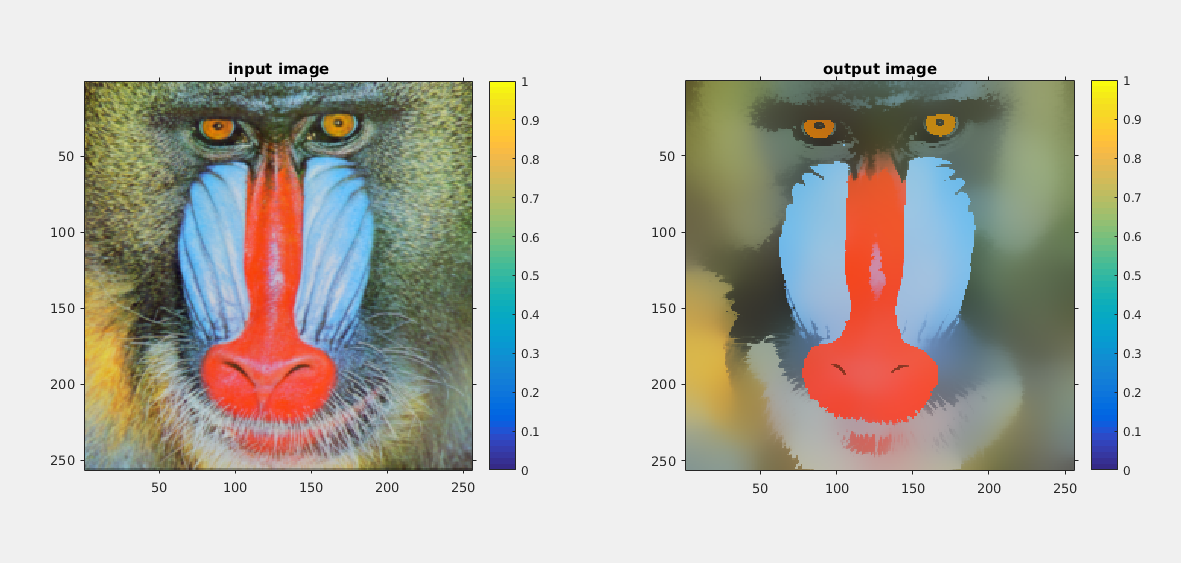
\includegraphics[width=\linewidth]{without_bin.png}
  \caption{Derivative image, corresponding to the derivative along the X axis}  
  \label{fig:result1}
\end{figure}


\begin{figure}[h!]
  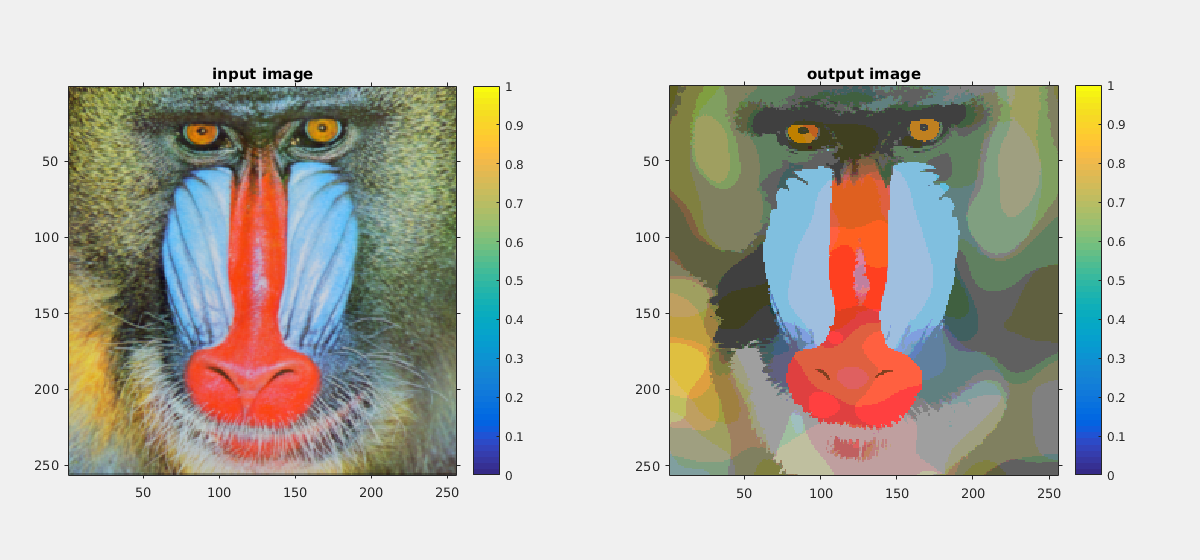
\includegraphics[width=\linewidth]{with_bin.png}
  \caption{Derivative image, corresponding to the derivative along the Y axis}
  \label{fig:result2}
\end{figure}

\begin{figure}[h!]
  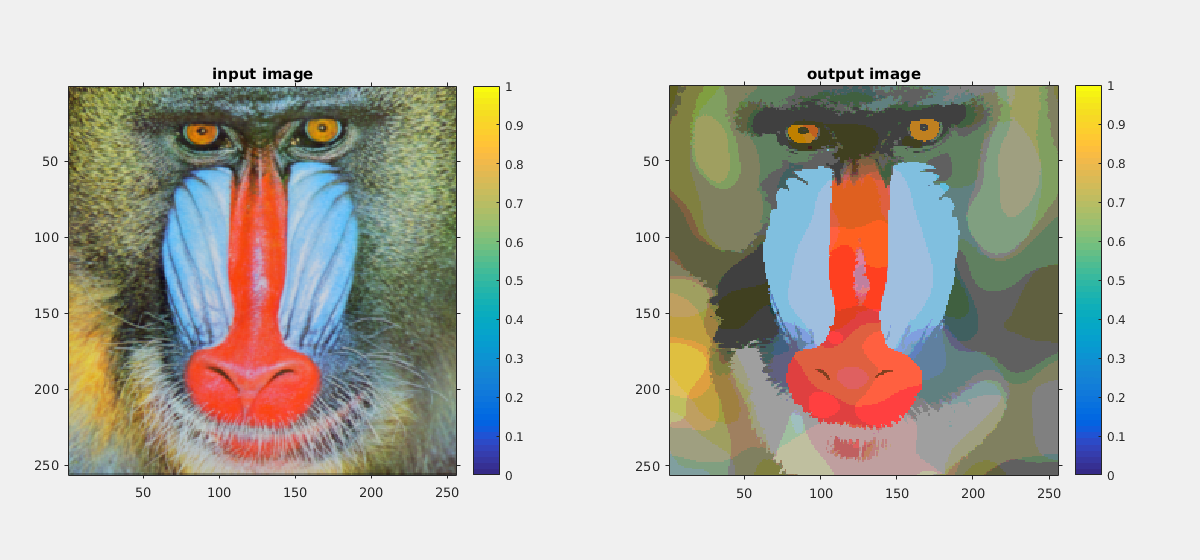
\includegraphics[width=\linewidth]{with_bin.png}
  \caption{Eigenvalue 1}
  \label{fig:result2}
\end{figure}

\begin{figure}[h!]
  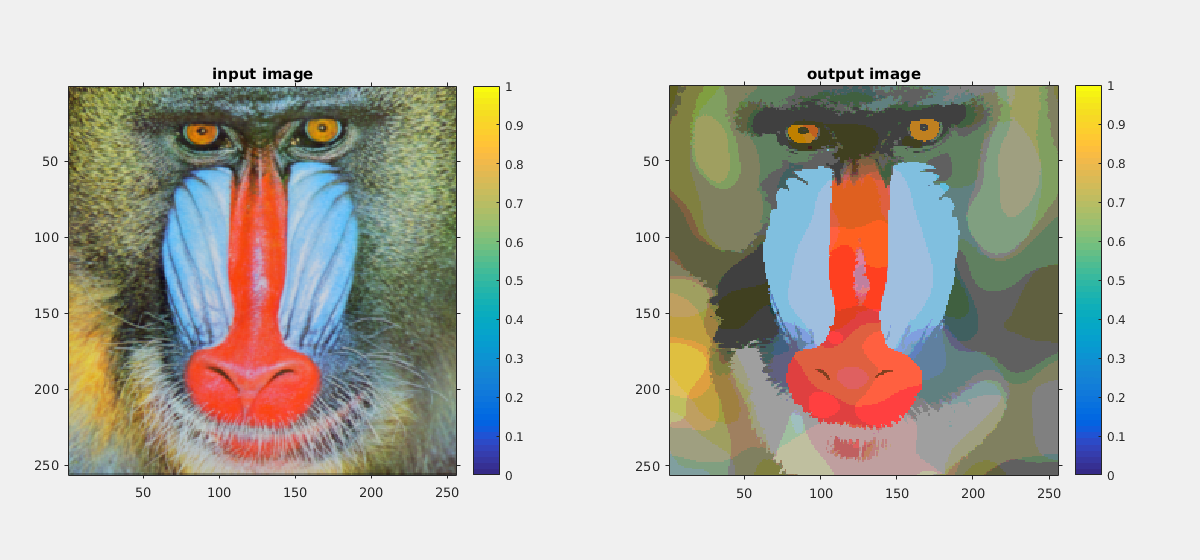
\includegraphics[width=\linewidth]{with_bin.png}
  \caption{Eigenvalue 2}
  \label{fig:result2}
\end{figure}


\begin{figure}[h!]
  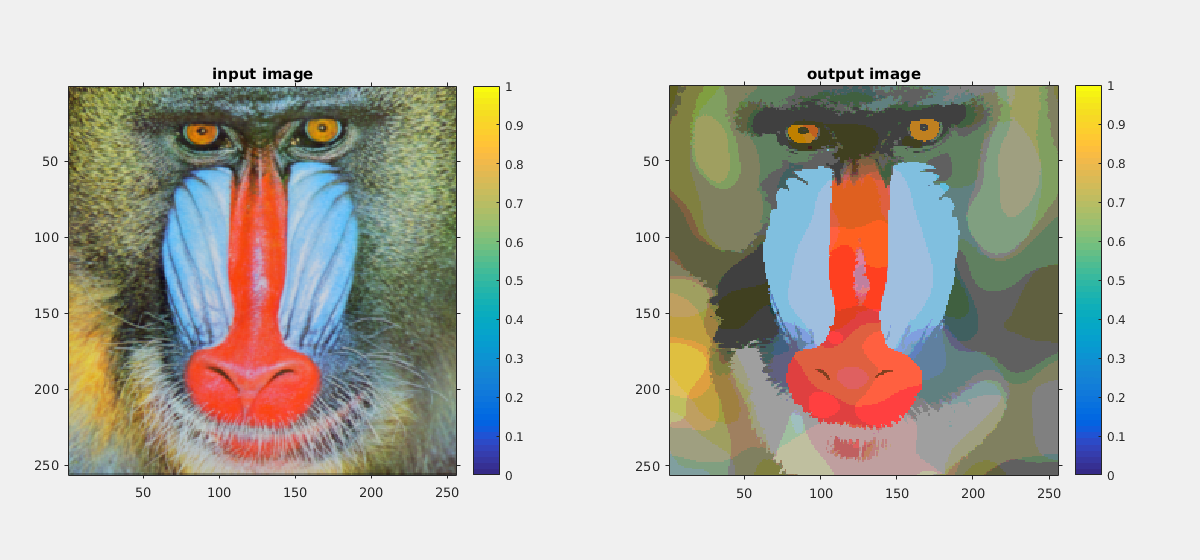
\includegraphics[width=\linewidth]{with_bin.png}
  \caption{Harris corner-ness measure image}
  \label{fig:result2}
\end{figure}

\begin{figure}[h!]
  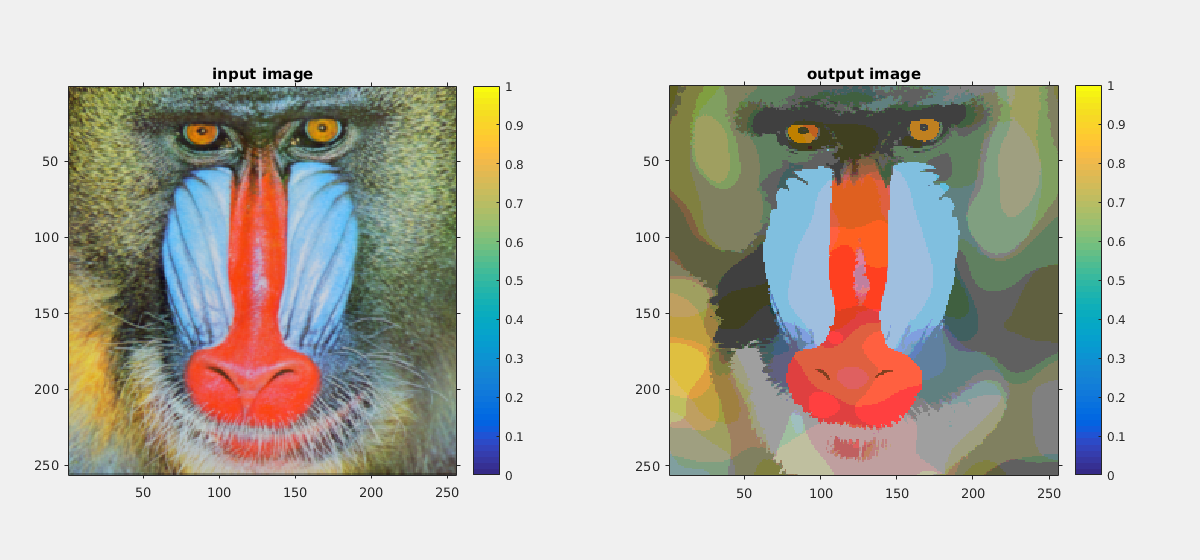
\includegraphics[width=\linewidth]{with_bin.png}
  \caption{Final Output without Non-Maximal Suppression}
  \label{fig:result2}
\end{figure}


\begin{figure}[h!]
  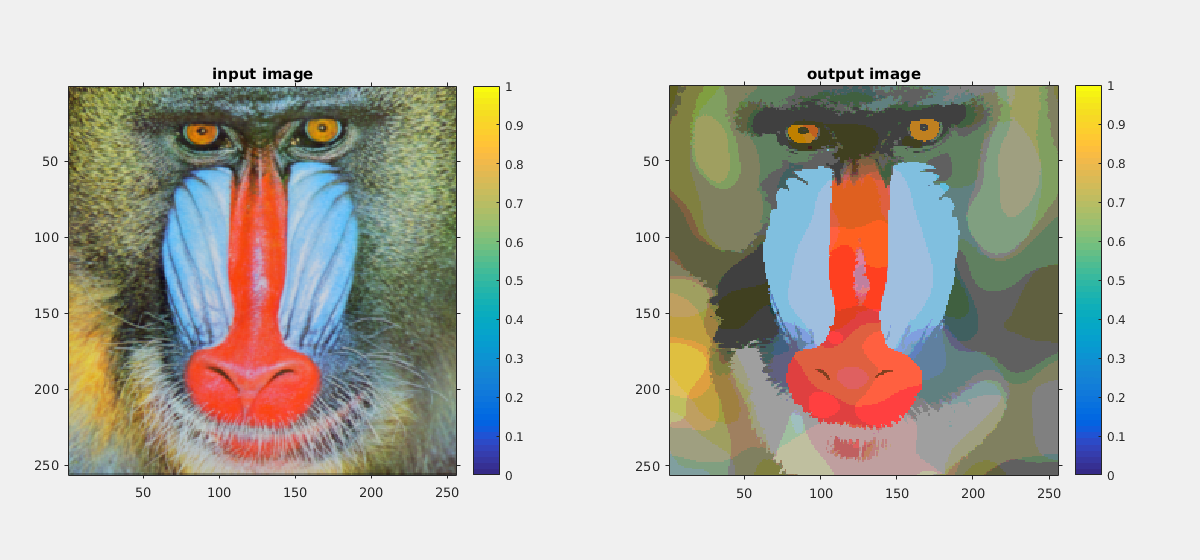
\includegraphics[width=\linewidth]{with_bin.png}
  \caption{Final Output with Non-Maximal Suppression}
  \label{fig:result2}
\end{figure}


\newpage

\textbf{Sigma in gaussian smoothing of input image } \texttt{= 0.2} \newline
\textbf{Sigma in gaussian smoothing of images of derivatives } \texttt{= 0.5} \newline
\textbf{K }(constant  in the measure of cornerness)\texttt{= 0.15} \newline
\textbf{We have thresholded the cornerness to} \texttt{0.011}

\end{document}